%================================================================================================
%================================= PRIMEIRA FOLHA INTERNA  ======================================
%================================================================================================
\begin{figure}
\center

\includegraphics[height=0.15\textwidth]{Figs/logoCefetCampusPetropolis.jpg} 
\end{figure}


\vspace*{0.8cm}

\begin{center}
{\large \bf CENTRO FEDERAL DE EDUCAÇÃO TECNOLÓGICA} \vspace{1mm} \\
{\large \bf CELSO SUCKOW DA FONSECA - CEFET/RJ \textit{CAMPUS} PETRÓPOLIS} \vspace{1mm} \\
{\large \bf CURSO: BACHARELADO EM ENGENHARIA DA COMPUTAÇÃO}\\

\vspace*{5cm}
{\large \bf PREVISÃO NEURAL DE TENDÊNCIAS DE VALORES FUTUROS DO BITCOIN}\\
\end{center}
\vspace{4cm}
\hfill
%\begin{minipage}%{0.45\linewidth}
	\begin{flushright}
	Bernardo Botelho Antunes da Costa
	\end{flushright}
%\end{minipage}


\vspace*{3.3cm}
\begin{center}
{\bf PETRÓPOLIS \\ 2018}\\
\end{center}

%--------------------------------------------------------------------------
%--------------------------------------------------------------------------
\newpage
\pagestyle{empty}

\begin{center}
{\large \bf CENTRO FEDERAL DE EDUCAÇÃO TECNOLÓGICA} \vspace{1mm} \\
{\large \bf CELSO SUCKOW DA FONSECA - CEFET/RJ \textit{CAMPUS} PETRÓPOLIS} \vspace{1mm} \\
{\large \bf CURSO: BACHARELADO EM ENGENHARIA DA COMPUTAÇÃO}

\vspace*{3cm}
\normalsize{\large \bf PREVISÃO NEURAL DE TENDÊNCIAS DE VALORES FUTUROS DO BITCOIN}\\
\end{center}
\vspace{1.5cm}
\hfill
%\begin{minipage}%{0.45\linewidth}
	\begin{flushright}
	Bernardo Botelho Antunes da Costa
	\end{flushright}
%\end{minipage}
\vspace*{1.5cm}
\begin{flushright}
	\begin{minipage}{0.5\textwidth}
		{\normalsize
		Trabalho de Conclusão de Curso apresentado ao  
	 CEFET/RJ -{\it campus} Petrópolis, como parte dos requisitos para obtenção do título de Bacharel em Engenharia da Computação.}
	\end{minipage}\\[1.5cm]
\end{flushright}
\vspace{1.5cm}
\hfill
%\begin{minipage}%{0.45\linewidth}
\begin{flushright}
Orientador: Prof. Diego Barreto Haddad, D.Sc.
\end{flushright}




\vspace*{3.3cm}
\begin{center}
{\bf PETRÓPOLIS \\ 2018}\\
\end{center}



%--------------------------------------------------------------------------
%--------------------------------------------------------------------------
\newpage
\begin{minipage}{0.9\textwidth}

{\normalsize 
\begin{center}
Autorizo(amos) a reprodução e divulgação total ou parcial deste trabalho, por qualquer meio
eletrônico ou convencional, para fins de estudo e pesquisa, desde que citada a fonte.
\end{center}
\vspace*{0.5cm}
}
\end{minipage}
\vspace*{5cm}
\begin{center}
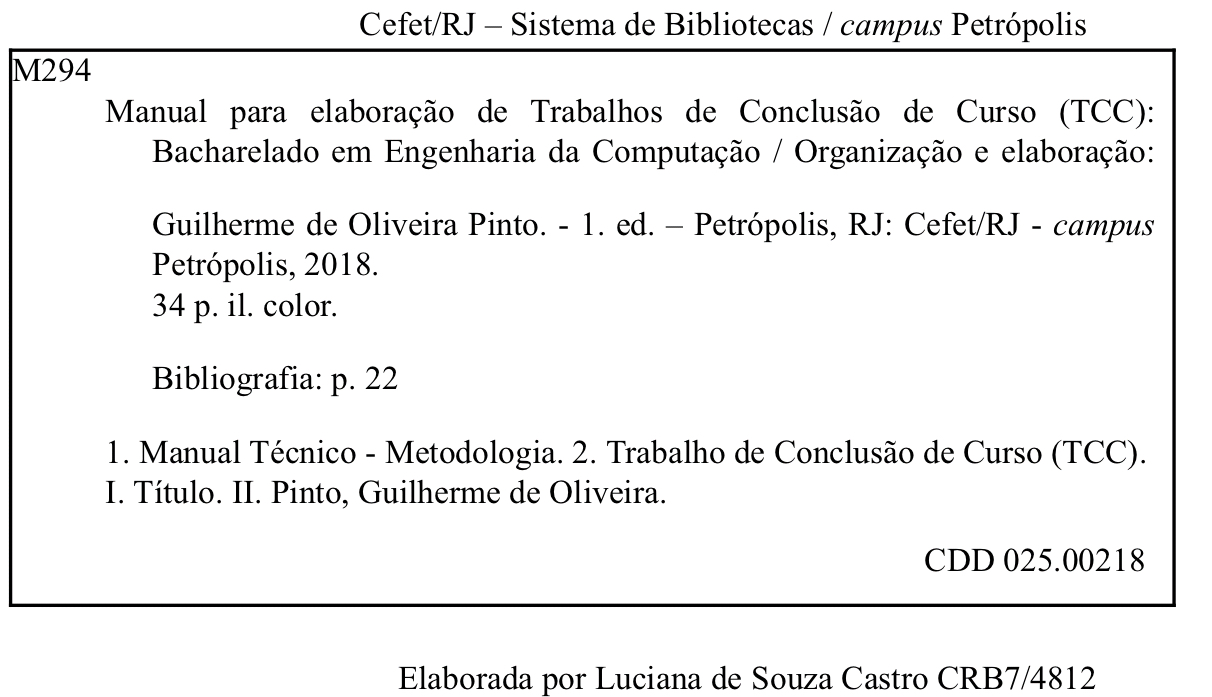
\includegraphics[height=0.4\textwidth]{Figs/biblioteca_engcomp.jpeg} 
\end{center}






%--------------------------------------------------------------------------
%--------------------------------------------------------------------------

\newpage
\newcommand{\HRule}{\rule{0.6\linewidth}{0.5mm}}
\pagestyle{empty}

{\center % Center everything on the page


\begin{figure}
\center

\includegraphics[height=0.13\textwidth]{Figs/logoCefetCampusPetropolis.jpg} 
\end{figure}

\begin{center}
{\large \bf CENTRO FEDERAL DE EDUCAÇÃO TECNOLÓGICA} \vspace{1mm} \\
{\large \bf CELSO SUCKOW DA FONSECA - CEFET/RJ \textit{CAMPUS} PETRÓPOLIS} \vspace{1mm} \\
{\large \bf CURSO: BACHARELADO EM ENGENHARIA DA COMPUTAÇÃO}\\
\vspace*{1.2cm}
{\large  FOLHA DE APROVAÇÃO}

\vspace*{1.3cm}
{\large \bf  Previsão Neural de Tendência de Valores Futuros do Bitcoin}\\
\end{center}
\vspace{0.5cm}
\hfill
%\begin{minipage}%{0.45\linewidth}
\begin{flushright}
    Bernardo Botelho Antunes da Costa
	\end{flushright}
%\end{minipage}
\vspace*{0.5cm}
\begin{flushright}
	\begin{minipage}{0.5\textwidth}
		{\normalsize
		Trabalho de Conclusão de Curso apresentado ao  
	 CEFET/RJ -{ {\it campus} Petrópolis}, como parte dos requisitos para obtenção do título de Bacharel em Engenharia da Computação.}
	\end{minipage}\\[0.5cm]
\end{flushright}
\vspace{0.5cm}
\hfill
%\begin{minipage}%{0.45\linewidth}
\begin{flushright}
Orientadora: Profa. Margaret Hamilton
\end{flushright}

\begin{minipage}{0.9\textwidth}
	\begin{flushleft}
	Aprovado por:
	\end{flushleft}
\end{minipage}\\[1cm]

\center
\HRule \\
Prof. Diego Barreto Haddad, D.Sc. (Orientador) \\[0.4cm]
\HRule \\
Prof. Luis Domingues Tomé Jardim Tarrataca, D.Sc.\\[0.4cm]
\HRule \\
Prof. Que o Diego escolher, D.Sc.  \\[1.5cm]


\begin{center}
{Agosto de 2018}
\end{center}


}



\newpage


% Dedicat�ria
%\begin{center}
%\textbf{\large DEDICATÓRIA}
%\end{center}
%      \vspace{0.5cm}
%
%Opcional.
%\newpage



% Agradecimento
\begin{center}
\textbf{\large  AGRADECIMENTO}
\end{center}
      \vspace{0.5cm}

Dedico este trabalho ao povo brasileiro que contribuiu de forma significativa a minha formação e estada nesta Universidade. Este projeto é uma pequena forma de retribuir o investimento e confiança em mim depositados.



\newpage


% Resumo
\begin{center}
\textbf{\large RESUMO}
\end{center}
      \vspace{0.5cm}

Inserir o resumo do seu trabalho aqui.

\begin{flushleft}
{\bf Palavras-chaves:} Previsão. Bitcoin. Google Trends. Redes neurais.
\end{flushleft}

\newpage

\begin{center}
\textbf{\large ABSTRACT}
\end{center}
\vspace{0.5cm}

Inserir o resumo do trabalho aqui, na Língua Inglesa.


\begin{flushleft}
{\bf Key-words:} Forecasting. Bitcoin. Google Trends. Neural Networks.
\end{flushleft}
